% Options for packages loaded elsewhere
\PassOptionsToPackage{unicode}{hyperref}
\PassOptionsToPackage{hyphens}{url}
\PassOptionsToPackage{dvipsnames,svgnames,x11names}{xcolor}
%
\documentclass[
  letterpaper,
  DIV=11,
  numbers=noendperiod]{scrartcl}

\usepackage{amsmath,amssymb}
\usepackage{setspace}
\usepackage{iftex}
\ifPDFTeX
  \usepackage[T1]{fontenc}
  \usepackage[utf8]{inputenc}
  \usepackage{textcomp} % provide euro and other symbols
\else % if luatex or xetex
  \usepackage{unicode-math}
  \defaultfontfeatures{Scale=MatchLowercase}
  \defaultfontfeatures[\rmfamily]{Ligatures=TeX,Scale=1}
\fi
\usepackage{lmodern}
\ifPDFTeX\else  
    % xetex/luatex font selection
    \setmainfont[]{Palatino}
    \setsansfont[]{Optima}
\fi
% Use upquote if available, for straight quotes in verbatim environments
\IfFileExists{upquote.sty}{\usepackage{upquote}}{}
\IfFileExists{microtype.sty}{% use microtype if available
  \usepackage[]{microtype}
  \UseMicrotypeSet[protrusion]{basicmath} % disable protrusion for tt fonts
}{}
\usepackage{xcolor}
\setlength{\emergencystretch}{3em} % prevent overfull lines
\setcounter{secnumdepth}{-\maxdimen} % remove section numbering
% Make \paragraph and \subparagraph free-standing
\makeatletter
\ifx\paragraph\undefined\else
  \let\oldparagraph\paragraph
  \renewcommand{\paragraph}{
    \@ifstar
      \xxxParagraphStar
      \xxxParagraphNoStar
  }
  \newcommand{\xxxParagraphStar}[1]{\oldparagraph*{#1}\mbox{}}
  \newcommand{\xxxParagraphNoStar}[1]{\oldparagraph{#1}\mbox{}}
\fi
\ifx\subparagraph\undefined\else
  \let\oldsubparagraph\subparagraph
  \renewcommand{\subparagraph}{
    \@ifstar
      \xxxSubParagraphStar
      \xxxSubParagraphNoStar
  }
  \newcommand{\xxxSubParagraphStar}[1]{\oldsubparagraph*{#1}\mbox{}}
  \newcommand{\xxxSubParagraphNoStar}[1]{\oldsubparagraph{#1}\mbox{}}
\fi
\makeatother


\providecommand{\tightlist}{%
  \setlength{\itemsep}{0pt}\setlength{\parskip}{0pt}}\usepackage{longtable,booktabs,array}
\usepackage{calc} % for calculating minipage widths
% Correct order of tables after \paragraph or \subparagraph
\usepackage{etoolbox}
\makeatletter
\patchcmd\longtable{\par}{\if@noskipsec\mbox{}\fi\par}{}{}
\makeatother
% Allow footnotes in longtable head/foot
\IfFileExists{footnotehyper.sty}{\usepackage{footnotehyper}}{\usepackage{footnote}}
\makesavenoteenv{longtable}
\usepackage{graphicx}
\makeatletter
\def\maxwidth{\ifdim\Gin@nat@width>\linewidth\linewidth\else\Gin@nat@width\fi}
\def\maxheight{\ifdim\Gin@nat@height>\textheight\textheight\else\Gin@nat@height\fi}
\makeatother
% Scale images if necessary, so that they will not overflow the page
% margins by default, and it is still possible to overwrite the defaults
% using explicit options in \includegraphics[width, height, ...]{}
\setkeys{Gin}{width=\maxwidth,height=\maxheight,keepaspectratio}
% Set default figure placement to htbp
\makeatletter
\def\fps@figure{htbp}
\makeatother

\usepackage{booktabs}
\usepackage{longtable}
\usepackage{array}
\usepackage{multirow}
\usepackage{wrapfig}
\usepackage{float}
\usepackage{colortbl}
\usepackage{pdflscape}
\usepackage{tabu}
\usepackage{threeparttable}
\usepackage{threeparttablex}
\usepackage[normalem]{ulem}
\usepackage{makecell}
\usepackage{xcolor}
\usepackage{siunitx}

    \newcolumntype{d}{S[
      table-align-text-before=false,
      table-align-text-after=false,
      input-symbols={-,\*+()}
    ]}
  
\KOMAoption{captions}{tableheading}
\makeatletter
\@ifpackageloaded{caption}{}{\usepackage{caption}}
\AtBeginDocument{%
\ifdefined\contentsname
  \renewcommand*\contentsname{Table of contents}
\else
  \newcommand\contentsname{Table of contents}
\fi
\ifdefined\listfigurename
  \renewcommand*\listfigurename{List of Figures}
\else
  \newcommand\listfigurename{List of Figures}
\fi
\ifdefined\listtablename
  \renewcommand*\listtablename{List of Tables}
\else
  \newcommand\listtablename{List of Tables}
\fi
\ifdefined\figurename
  \renewcommand*\figurename{Figure}
\else
  \newcommand\figurename{Figure}
\fi
\ifdefined\tablename
  \renewcommand*\tablename{Table}
\else
  \newcommand\tablename{Table}
\fi
}
\@ifpackageloaded{float}{}{\usepackage{float}}
\floatstyle{ruled}
\@ifundefined{c@chapter}{\newfloat{codelisting}{h}{lop}}{\newfloat{codelisting}{h}{lop}[chapter]}
\floatname{codelisting}{Listing}
\newcommand*\listoflistings{\listof{codelisting}{List of Listings}}
\makeatother
\makeatletter
\makeatother
\makeatletter
\@ifpackageloaded{caption}{}{\usepackage{caption}}
\@ifpackageloaded{subcaption}{}{\usepackage{subcaption}}
\makeatother

\ifLuaTeX
  \usepackage{selnolig}  % disable illegal ligatures
\fi
\usepackage[style=apa]{biblatex}
\addbibresource{RethinkingEthnicity.bib}
\usepackage{bookmark}

\IfFileExists{xurl.sty}{\usepackage{xurl}}{} % add URL line breaks if available
\urlstyle{same} % disable monospaced font for URLs
\hypersetup{
  pdftitle={Resistance is Not Futile: Rethinking Ethnicity, Tactics, and Outcomes in Civil Conflicts},
  pdfauthor={Robert Tanner Bivens; Ches Thurber},
  colorlinks=true,
  linkcolor={blue},
  filecolor={Maroon},
  citecolor={Blue},
  urlcolor={Blue},
  pdfcreator={LaTeX via pandoc}}


\title{Resistance is Not Futile: Rethinking Ethnicity, Tactics, and
Outcomes in Civil Conflicts}
\author{Robert Tanner Bivens \and Ches Thurber}
\date{2026-03-24}

\begin{document}
\maketitle
\begin{abstract}
Recent studies have questioned whether nonviolent tactics can be
effective for ethnic minorities. However, they often overlook
multiethnic coalitions, shifts in campaign composition, and ethnicity's
parallel role in armed tactics. This paper re-evaluates the relationship
between ethnicity, tactics, and outcomes in civil conflicts. To do so,
we introduce new data on Ethnic Groups in Contention (EGC) that offer
time-variant measures of the ethnic attributes of campaigns. We find
that the effectiveness of nonviolent tactics for ethnic minorities
depends on the point of comparison. Campaigns composed solely of
excluded groups succeed less often than those made up entirely of
privileged groups. However, minorities have still fared better when
using nonviolent as compared to violent tactics. Additional analyses
explore ethnic diversity, multiethnic coalitions, hybrid tactics, and
alternative measures of success. Taken together, our findings complicate
a prevailing assertion that nonviolent tactics are only effective for
members of privileged groups.
\end{abstract}


\setstretch{2}
\textbf{Keywords:} Nonviolent Resistance, Civil War, Ethnic Conflict,
Social Movements

\begin{itemize}
\tightlist
\item
  Corresponding author: Ches Thurber, Department of Political Science,
  Northern Illinois University, cthurber@niu.edu.
\end{itemize}

Accepted for publication at the \emph{Journal of Peace Research.}

\section{Author Bios}\label{author-bios}

ROBERT TANNER BIVENS, b. 1989, PhD in Political Science (Northern
Illinois University, 2024); Instructor, Department of Political Science,
Eastern Illinois University (2024-Present); research interests:
sub-Saharan African politics, comparative regionalism, non-democratic
governance.

CHES THURBER, b. 1982, PhD in International Relations (Tufts University,
2015); Associate Professor, Department of Political Science, Northern
Illinois University (2016-- ); most recent book: \emph{Between Mao and
Gandhi: The Social Roots of Civil Resistance} (Cambridge University
Press, 2021).

\newpage

\section{Introduction}\label{introduction}

In several real-world cases, movements representing ethnic minorities,
from Black South Africans to Nepal's indigenous nationalities, have
abandoned nonviolent methods in favor of violence after coming to
believe that nonviolent tactics could not work for them
\autocite{Thurber2021}. Their decisions align with broader intellectual
critiques of nonviolent resistance as ineffective and even dangerous for
members of ethnic and racial minorities
\autocite{Gelderloos2007,CobbJr.2015,Jackson2020}.

A recent wave of scholarship has offered empirical support for those
critiques. Despite the widely celebrated finding that nonviolent tactics
have achieved higher rates of success than violent tactics in
overthrowing regimes \autocite{Chenoweth2011,Gleditsch2022}, several
studies have shown that success rates are far lower when an ethnic
cleavage distinguishes the movement from the regime
\autocite{Svensson2011,Pischedda2020}. One major work even found that
for ethnic minorities, nonviolent tactics are no more effective than
violence \autocite[161]{Manekin2022}.

Yet the research on the question of ethnicity and tactics falls short of
a consensus. Chenoweth and Stephan, for example, argue that ethnic
diversity should make a campaign more effective
\autocite{Chenoweth2011}, while Cunningham finds that a greater reliance
on nonviolent tactics is associated with a higher likelihood of success
among ethnic self-determination movements \autocite{Cunningham2023}.

The varied results reflect differences in how the studies conceptualize
ethnicity, in the types of goals being examined, and in the benchmarks
for comparison being used. Furthermore, nearly all prior studies have
been hindered by limited data, forcing them to treat ethnicity as a
static and binary dichotomy. This has prevented them from being able to
evaluate different dimensions of ethnicity, to consider the effects of
inter-ethnic coalitions, or to account for changes in campaign tactics
and ethnic composition over time.

This paper seeks to systematically reevaluate our knowledge of the
relationship between ethnicity, tactics, and outcomes in conflict. We
theorize the distinct roles of ethnic diversity and power status in
shaping the trajectories and outcomes of conflict, considering which of
these dynamics are likely to be universal and which are instead
conditional upon the tactics employed by the campaign. To test our
arguments, we introduce new data on Ethnic Groups in Contention
(EGC).\footnote{This version of the dataset, which we are calling EGC
  2.1, updates a prior version published by Thurber
  \autocite*{Thurber2018}. It expands upon that dataset by using the
  more recently published NAVCO 2.1 dataset for units of analysis and by
  offering yearly measures that are able to capture changes in
  campaigns' ethnic composition over time.} The data links ethnic groups
in the Ethnic Power Relations dataset \autocite{Vogt2015} to campaigns
from the NAVCO 2.1 dataset \autocite{Chenoweth2022}. We provide
time-variant measures of which ethnic groups participated in a given
campaign in each year. This allows us to both account for changes over
time, as well as to capture more precise concepts of ethnicity, such as
how many different groups participated, the size of those groups, their
geographic location, and whether those groups were politically included,
excluded, or both. We then conduct a series of descriptive and
regression analyses of the varied nature of ethnicity in both violent
and nonviolent campaigns and how these ethnic attributes of campaigns
relate to outcomes.

Our results confirm those of some prior studies, while challenging
others. Consistent with prior work, we find that campaigns are more
likely to be successful when they include participation from higher
status ethnic groups. However, we find that all types of campaigns, even
those made up entirely of politically excluded ethnic groups, have
experienced greater success when using nonviolent as compared to violent
tactics. We argue that this is because nonviolent tactics still confer
some of the same advantages for marginalized groups as they do for
ethnic majorities, while violent tactics offer little advantage in
overcoming the particular challenges marginalized groups face.

We also assess the impact of ethnic diversity, and find that a greater
number of participating ethnic groups is associated with higher rates of
success, but only when nonviolent tactics are used. Furthermore, we
recognize that past research has also been limited by narrow
conceptualizations of ``nonviolence'' and ``success''
\autocite{Turner2023,Cunningham2023}. We therefore explore the use of
hybrid tactics as well as alternative thresholds of success in the
latter sections of the paper. We find that campaigns made up entirely of
minorities are just as likely as those with privileged groups to achieve
concessions short of wholesale regime change or secession. We observe no
difference in outcomes between campaigns that employ hybrid strategies
and those that maintain more strict nonviolent discipline.

As with all observational studies on tactical effectiveness in conflict,
our results are vulnerable to the problem of selection bias. In the main
text and an appendix, we discuss the most likely sources of endogeneity,
run year- and country-level fixed effects models to account for omitted
variables that might be correlated with those units, and present
sensitivity analyses. These are far from a cure-all for the problem of
selection bias, but they allow us to better assess the potential
direction and degree of the problem and to contextualize our
interpretations accordingly. Most crucially, our findings should be
understood as those that emerge from within the set of campaigns that
are able to meet the NAVCO dataset's selection criteria of mobilizing at
least 1,000 participants.

Given the impact of previous observational findings on ethnicity in
civil resistance campaigns to scholarly debates as well as to public
discourse, we believe that the more detailed scrutiny of the historical
data offered by this paper is needed.

\section{Ethnicity and the Outcomes of Violent and Nonviolent
Campaigns}\label{ethnicity-and-the-outcomes-of-violent-and-nonviolent-campaigns}

Underpinning theories of the impact of ``ethnicity'' on conflict are
distinct mechanisms that link different dimensions of ethnicity to
specific conflict dynamics. Some theories highlight the advantages of
ethnic heterogeneity on building mass resistance and making repression
difficult \autocite{Chenoweth2011}. Others emphasize the challenges that
come from exclusion from institutions of political power or from small
demographic size \autocite{Thurber2018,Pischedda2020}. And others still
focus on social connections or shared identity frames between
participants and those on the sidelines
\autocite{Svensson2011,Manekin2022} .

In most cases, prior work has relied on a simplified dichotomy,
considering conflicts to either be inherently ``ethnic'' or ``not
ethnic'' along some prescribed criteria. Pischedda
\autocite*{Pischedda2020} focuses on whether or not an ethnic
``cleavage'' exists between protesters and regime. Thurber
\autocite*{Thurber2018} and Manekin and Mitts \autocite*{Manekin2022}
assess the demographic size of a campaign's leading ethnic group as well
as its power status. Each of these conceptualizations has unique
theoretical as well as empirical implications. Conceptually, they all
struggle to deal with movements that comprise multiple groups.
Operationally, they do not account for changes in the ethnic composition
of movements over time. And theoretically, they do not consider whether
or not similar obstacles may exist for marginalized groups using armed
tactics.

In the section that follows, we untangle these distinct logics,
considering how various dimensions of ethnicity are likely to impact the
trajectories and outcomes of campaigns across tactics, as well as
whether the relative efficacy of nonviolent versus violent tactics is
contingent on ethnicity.

\subsection{\texorpdfstring{\textbf{Ethnic Power Status and Campaign
Outcomes}}{Ethnic Power Status and Campaign Outcomes}}\label{ethnic-power-status-and-campaign-outcomes}

A major step in the study of ethnic conflict was the move away from
demographic measures of ethnicity and toward measures that better
account for the power relationships between various ethnic groups and
the state \autocite{Cederman2007,Wimmer2009}. The Ethnic Power Relations
project, for example, identified inclusion versus exclusion from
political power as a key ethnopolitical dynamic with implications for
civil conflict \autocite{Cederman2010,Vogt2015}. However, much of the
focus remained on how ethnic exclusion produces grievances that spark
conflict as opposed to how it shapes conflict outcomes.

Thurber \autocite*{Thurber2018} and Pischedda \autocite*{Pischedda2020}
both argue that ethnic power relationships underpin dynamics central to
the strategic logic of nonviolent conflict. They show that when the
participants in a campaign are excluded from holding positions of power
in the state, it makes it easier for the regime to engage in repression
and less likely that regime elites will defect and join the opposition.
In fact, Pischedda finds that an ethnic cleavage in a nonviolent
conflict is negatively correlated with both civilian as well as security
force defections. Exclusion from security forces is likely to impact
dynamics of repression as well. With fewer fears of defections and fewer
ties to the opposition, security forces will be more willing to use
deadly force against unarmed protesters when those protesters are from a
different ethnic group.

Meanwhile, a campaign comprised only of marginalized ethnic groups
alleviates the discrimination problem for state forces, making it easier
for the regime to infer loyalty on the basis of ethnicity. Only when
members of politically privileged ethnic groups are participating in the
resistance does the state face the most acute risk of ``backfire,'' in
which efforts to repress dissent drive neutrals or loyalists into the
arms of the opposition \autocite{Martin2007}. This logic produces the
prediction that nonviolent campaigns that are made up of only members of
excluded ethnic groups will be less likely to achieve success than those
that include members of incumbent groups.

Prior work has not given much attention to the dynamics of campaigns
that include both incumbent and excluded ethnic groups. An important
exception is Manekin, Mitts, and Zeira \autocite*{Manekin2024}, who find
that the presence of more privileged ``allies'' offers advantages to
minority-led movements by increasing popular approval, perceptions of
nonviolence, and willingness to participate among members of privileged
groups. The logic of Thurber \autocite*{Thurber2018} and Pischedda
\autocite*{Pischedda2020} would also suggest that the participation of a
privileged group should increase the prospects for success by providing
social connections to the regime. Furthermore, the presence of members
of an incumbent group within the campaign complicates efforts at
identifying and targeting dissidents.

However, it is also possible that the mere presence of a marginalized
group in a campaign, even when alongside participation from a more
powerful group, can trigger negative consequences for the campaign. In
the context of the 2011 Syrian uprising, McLauchlin
\autocite*{McLauchlin2017}, notes that even though members of the
dominant Alawite group participated, the large presence of Sunnis in the
movement allowed the regime to stoke ethnic fears, undermining the
movement's perceived legitimacy and building support for brutal
repression.

Given this confluence of competing dynamics, we expect these cases of
mixed participation to experience rates of success somewhere in the
middle: lower than campaigns made up entirely of members of incumbent
groups, but higher than campaigns made up entirely of excluded groups.

The arguments above draw primarily from scholarship focusing on the role
of ethnic power status in nonviolent conflicts. But both theory and
prior empirical research suggest that minorities engaged in armed
insurrection may face similar impediments. While civil war scholarship
has generally been more focused on etiology than outcomes, quantitative
studies that have analyzed the link between ethnicity and effectiveness
have found rebel victory to be substantially less likely when a war is
``ethnic'' versus ``non-ethnic'' \autocite{Mason1996,deRouen2004}.

Why is this the case? Some of the same mechanisms cited in the
literature on civil resistance likely apply to insurgencies as well. For
example, the relationship between ethnicity and defections highlighted
in the nonviolent conflict literature has also been noted in civil war
scholarship. Armed rebellions by ``in-groups'' are more likely to
splinter state security forces, creating greater opportunity for
success, while rebellions by excluded minorities are less likely to
challenge the loyalty of the military \autocite{McLauchlin2010}.
Meanwhile, the role of ethnicity as a marker to discern loyalty
originally comes from the armed conflict literature and is the
theoretical rationale behind Mason, Weingarten, and Fett's finding that
ethnic rebellions experience lower rates of victory
\autocite*[263]{Mason1996}.

Some ethnic dynamics may impact unarmed tactics to a greater degree than
armed ones. We turn to a discussion of these relative differences in the
next section. But because marginalized status creates obstacles for
excluded ethnic groups both when they use violence as well as
nonviolence, we expect the association between ethnic status and success
to exist across both tactical repertoires.

\begin{quote}
\textbf{H1:} \emph{Campaigns involving ethnic groups with higher levels
of political power will be more likely to succeed, regardless of tactics
used.}
\end{quote}

\subsection{\texorpdfstring{\textbf{Is the nonviolent advantage
conditional on
ethnicity?}}{Is the nonviolent advantage conditional on ethnicity?}}\label{is-the-nonviolent-advantage-conditional-on-ethnicity}

The previous section advanced the argument that excluded ethnic groups
will face lower odds of success whether they employ primarily armed or
unarmed methods. But is there still an advantage to using nonviolent
tactics for politically excluded groups?

Manekin and Mitts argue that in-groups tend to view any resistance by
members out-groups as ``violent,'' thereby negating the advantages of
adhering to nonviolent tactics \autocite[162]{Manekin2022}. But even
with notable disadvantages as compared to incumbent groups, excluded
minorities may still be able to harness many of the benefits of a
nonviolent strategy. Ethnic biases may prevent local audiences from
viewing minority protest favorably, but an adherence to primarily
nonviolent tactics might help such a movement gain international
support. Such support was critical, for example, in the end of the
Apartheid regime in South Africa.

And while ethnic cleavages are likely to be an impediment to mass
mobilization, unarmed tactics might better enable a movement to maximize
participation among co-ethnics and make it more likely to attract at
least some support across ethnic divides as compared to if dissidents
used violent force. Chenoweth and Stephan (2011) highlight both of these
dynamics in their analysis of why they believe the first Palestinian
intifada was more successful during the years in which it was primarily
nonviolent .

Finally, while excluded ethnic groups are likely to face greater
repression from the state, they are just as likely (if not more) to face
such repression if they took arms. When an excluded group adheres to
nonviolent tactics, it increases the cost of that repression to the
regime. Even if ethnic divisions limits local sympathy from privileged
ethnic groups, international actors may be more likely to intervene
\autocite{Cunningham2023}. For example, the Dilli Massacre of 1991
brought international support to the East Timorese movement, leading
eventually to a UN-sponsored referendum in 1999 and independence in
2002.

In sum, members of excluded ethnic groups engaged in nonviolent tactics
may struggle to mobilize, face greater repression, and more frequently
fail to win over elite defections as compared to members of incumbent
ethnic groups. But they struggle even more on these fronts when they use
violent tactics. Several case study analyses of minority resistance
movements in Palestine, South Africa, and East Timor, for example, have
concluded that those movements achieved relatively greater success
during periods of time in which they used primarily nonviolent tactics
\autocites[138-145]{Chenoweth2011}{Barrell1992,Zunes1999b,MacLeod2015,Stephan2008}.
This logic produces the following hypothesis.

\begin{quote}
\textbf{H2:} \emph{Campaigns using nonviolent tactics will be more
likely to succeed, regardless of participants' ethnic power status.}
\end{quote}

In Table 1, we bring together our theoretical predictions from
Hypotheses 1 and 2. We show that within each tactic, we expect groups
with higher ethnic status levels to enjoy higher rates of success, but
that across the board we expect success rates to be higher when
nonviolent tactics are used. We classify the ethnic composition of
campaigns into three status categories: ``Incumbents'' refers to
campaigns in which all participating ethnic groups have access to state
power, ``Excluded'' refers to campaigns in which all participating
ethnic groups are excluded from power, and ``Mixed'' refers to campaigns
in which at least one included and one excluded group are present.

\begin{longtable}[]{@{}lll@{}}
\caption{Predicted success rates based on ethnic status of participants
and tactics.}\tabularnewline
\toprule\noalign{}
\textbf{Ethnic Status} & \textbf{Nonviolent Tactics} & \textbf{Violent
Tactics} \\
\midrule\noalign{}
\endfirsthead
\toprule\noalign{}
\textbf{Ethnic Status} & \textbf{Nonviolent Tactics} & \textbf{Violent
Tactics} \\
\midrule\noalign{}
\endhead
\bottomrule\noalign{}
\endlastfoot
\textbf{Incumbents} & Highest & Low \\
\textbf{Mixed} & Higher & Lower \\
\textbf{Challengers} & High & Lowest \\
\end{longtable}

\subsection{\texorpdfstring{\textbf{Ethnic Diversity and Campaign
Success}}{Ethnic Diversity and Campaign Success}}\label{ethnic-diversity-and-campaign-success}

While the first two hypotheses focused on ethnic power status, Chenoweth
and Stephan's \autocite*{Chenoweth2011} landmark study highlighted a
different dimension of ethnicity: the ethnic \emph{diversity} of a
campaign. Greater diversity of participants may allow campaigns to tap
into more diffuse social networks and leverage a wider set of tactical
skills. Furthermore, a campaign with diverse participants may make
selective repression by the state more difficult. They write, ``The more
diverse the participation in the resistance--in terms of gender, age,
religion, ethnicity, ideology, profession, and socioeconomic status--the
more difficult it is for the adversary to isolate participants and adopt
a repression strategy short of maximum and indiscriminate repression''
\autocite[40]{Chenoweth2011}.

The argument parallels recent social movement research that highlights
the importance of inter-ethnic coalitions
\autocite{Dixon2013,Gawerc2020}. Looking beyond ethnicity, Sirianne
Dahlum \autocite*{Dahlum2023} finds that more socially heterogenous
civil resistance campaigns are more likely to be successful for similar
reasons.

While most discussions focus on either a presence or absence of
diversity, we should expect the participation of additional ethnic
groups (i.e.~three or more) to confer even greater benefits. The greater
the number of ethnic groups participating, the greater the potential for
mobilization and the thornier the challenge of identification on the
basis of ethnicity for the regime.

From these arguments, we draw the hypothesis that, for nonviolent
campaigns, a greater number of different ethnic groups in a campaign
will increase the likelihood for success:

\begin{quote}
\textbf{H3:} \emph{Among nonviolent campaigns, those with greater ethnic
diversity will be more likely to succeed.}
\end{quote}

Armed rebels might also benefit both from being able to recruit from
multiple subgroups of the population as well as from limiting the
state's ability to isolate insurgents' bases of support. But these
benefits are likely to be relatively less important given the diminished
centrality of mass participation to the strategic logic of insurgency.

Furthermore, studies of insurgency suggest that ethnic homogeneity can
be an asset to armed rebels. As Gubler and Selway
\autocite*[209]{Gubler2012} write, sharing a single ethnicity can form
the basis for identity-based fervor that can motivate individuals to
take on the greater risk of potentially lethal participation. It can
make it easier for rebel leaders to create and maintain social control
within the organization: for the guerrilla commander trying to coerce
high-risk mobilization, the strong ``bonding'' ties of insular networks
may be more beneficial than the ``bridging'' ties afforded by a more
diverse movement \autocite{Thurber2021}.

For armed conflicts, it is not clear whether diversity or homogeneity is
more advantageous. As such, we do not make a prediction about the
relationship between diversity and outcomes in violent conflicts.

\subsection{}\label{section}

\section{Measuring Ethnicity in Mass
Uprisings}\label{measuring-ethnicity-in-mass-uprisings}

Testing the hypotheses articulated above requires detailed data on the
role of ethnicity in mass uprisings. To date, only limited data has been
available. The Nonviolent and Violent Campaign Outcomes (NAVCO) datasets
include a binary measure of ethnic diversity
\autocite{Chenoweth2013,Chenoweth2022}. However, they do not
differentiate among campaigns with two or more groups participating, nor
do they account for dynamics of political power among ethnic groups.

In their analyses of the impact of ethnic cleavages on campaign
outcomes, both Svensson and Lindgren \autocite*{Svensson2011} as well as
Pischedda \autocite*{Pischedda2020} use a binary measure of whether or
not an ethnic cleavage exists between regime and dissidents. But they do
not provide information on exactly who is participating in the campaign.
They are not able to account for the number of different groups
participating, whether the campaign included participation from both
included and excluded ethnic groups, or whether dissidents are framing
claims in explicitly ethnic terms. They also code only campaigns using
primarily nonviolent tactics. The ACD2EPR dataset
\autocite{Wucherpfennig2012}, by contrast, only includes armed
conflicts.

We therefore collected new data on the ethnic attributes of mass
uprisings, identifying exactly which ethnic groups participated in the
campaign and whether ethnic claims were made. We use data from Thurber
\autocite*{Thurber2018} as a point of departure, but we update it in two
key respects. First, we use the more recent 2.1 version of the NAVCO
dataset to provide our units of analysis \autocite{Chenoweth2022}. This
dataset improves upon the prior version by including campaigns as recent
as 2013, adding previously omitted campaigns that meet the scope
criteria, and adding additional measures for each campaign. Second,
while earlier data only provided a snapshot of the ethnic composition at
the onset of a campaign, we provide yearly measures, accounting for
over-time change within a campaign. In fact, we find that nearly 10
percent of campaigns experience a change in their ethnic composition.

For each NAVCO 2.1 campaign-year, we identify specific ethnic groups
from the Ethnic Power Relations (EPR) 2019 dataset that participated in
the campaign \autocite{Vogt2015}. We rely on sources such as the ACD2EPR
dataset \autocite{Wucherpfennig2012}, the Swarthmore Global Nonviolent
Action Database \autocite{Lakey2011}, qualitative appendices from NAVCO
\autocite{Chenoweth2011}, and additional secondary sources to determine
which groups participated in a campaign. We rely on whether there are
reported accounts in the secondary literature of participation of a
given ethnic group in a campaign to make our coding decisions. This
approach is consistent with prior data, such as the ACD2EPR dataset.

From the list of participating ethnic groups, we produce more general
measures of ethnic attributes of each campaign at the yearly level. To
examine dynamics of ethnic power and coalition, we divide campaigns into
the three categorical types discussed previously: ``Incumbents'' include
only ethnic groups coded by EPR as having access to power, ``Excluded''
consist entirely of ethnic groups that are excluded from power, and
``Mixed'' feature participation by at least one included and and at
least one excluded ethnic group.

Our data also makes it possible to analyze other dimensions of ethnicity
in conflict that have not featured as prominently in recent studies. To
assess campaign diversity, we count the total number of groups
participating in the campaign. We also note whether or not any
participating ethnic group within a campaign makes an ethnic claim, that
is, if they articulate explicit political, economic, or social goals
that are specific to that ethnic group. Evidence of an ethnic claim
often comes in the name of a campaign organization (e.g.~``Tigray
People's Liberation Front''), or from publicly stated platforms that
reference the rights or grievances of a specific group.

Finally, by identifying the specific ethnic groups participating in a
campaign, we can incorporate additional data from the Ethnic Power
Relations project. This includes the demographic size of participation
groups, as well as geographic settlement patterns. Using GeoEPR data
\autocite{Wucherpfennig2011}, we assess whether any participating group
resides in primarily urban areas, as urban versus rural geography is
often considered to offer differing advantages to armed and unarmed
tactics. Additional information about our data collection and coding
procedures can be found in the Online Appendix.

While the NAVCO and EPR datasets provide a strong foundation for this
study, a few notes regarding the particularities of those datasets are
in order. The NAVCO dataset examines only cases of ``maximalist''
campaigns, essentially those seeking wholesale regime-change or
secession. We think this fits with our theoretical logic which is
centered on the presumption of resistance movements that present an
existential challenge to the regime and its sovereign control of the
territory of the state. It also only includes campaigns once they reach
a threshold of 1,000 participants. We discuss the potential for
selection bias created by this threshold later in the paper.

Meanwhile, the EPR dataset focuses on ethnic groups that it deems
``politically relevant.'' In some cases, it includes groups, but assigns
them a power status of ``Irrelevant.'' In order to include these cases
in our analysis, we attempt to assign them a status using procedures
described in detail in our Online Appendix (p.~6). We also run analyses
in which we omit these cases to demonstrate that they do not drive our
findings (Online Appendix, Table 11, p.~20).

\begin{table}
\centering\centering
\caption{Ethnic attributes of NAVCO 2.1 campaign-years.}
\centering
\resizebox{\ifdim\width>\linewidth\linewidth\else\width\fi}{!}{
\begin{tabular}[t]{llrrrr}
\toprule
\multicolumn{2}{c}{ } & \multicolumn{2}{c}{Nonviolent (N=510)} & \multicolumn{2}{c}{Violent (N=2207)} \\
\cmidrule(l{3pt}r{3pt}){3-4} \cmidrule(l{3pt}r{3pt}){5-6}
  &    & Mean & Std. Dev. & Mean & Std. Dev.\\
\midrule
Number of Groups &  & \num{1.6} & \num{1.2} & \num{2.0} & \num{2.2}\\
Population Share &  & \num{0.6} & \num{0.4} & \num{0.4} & \num{0.4}\\
Primary Urban Group &  & \num{0.4} & \num{0.5} & \num{0.3} & \num{0.5}\\
Any Ethnic Claim &  & \num{0.4} & \num{0.5} & \num{0.7} & \num{0.5}\\
\midrule
 &  & N & Pct. & N & Pct.\\
Status & Excluded & \num{128} & \num{25.1} & \num{1064} & \num{48.2}\\
 & Mixed & \num{122} & \num{23.9} & \num{355} & \num{16.1}\\
 & Incumbents & \num{214} & \num{42.0} & \num{578} & \num{26.2}\\
\bottomrule
\end{tabular}}
\end{table}

Table 2 presents descriptive statistics of the ethnic composition of
campaign-years, disaggregated by the primary tactics used. The average
number of ethnic groups participating in a campaign in a given year is
1.6 for nonviolent campaigns and 2.0 for violent ones. The larger
average number of groups in violent campaigns runs counter to the idea
that nonviolent campaigns attract more diverse participation. Instead,
it appears that nonviolent campaigns draw participation from slightly
larger ethnic groups on average. The mean share of a country's total
population made up of ethnic groups participating in a primarily
nonviolent campaign was 0.6 while for violent campaigns was 0.4.
Meanwhile, the percentage of campaigns where the primary ethnic group is
settled in an urban area is slightly higher among nonviolent as compared
to violent campaigns. There is a stark difference across campaign
tactics when we examine whether or not any participating groups made
ethnic claims. Over two-thirds of violent campaign-years feature ethnic
claims, while less than half of nonviolent campaign-years do.

There are also notable differences between violent and nonviolent
campaigns when it comes to the power status of participating ethnic
groups. As shown in Table 2, 42\% of campaign-years in which primarily
nonviolent tactics were used involved only Incumbents. Only a quarter
(25\%) were made up entirely of Excluded groups, while another quarter
(24\%) were Mixed. By contrast, nearly half of violent campaign-years
were comprised entirely of Excluded groups. Incumbents account for about
a quarter (26\%) of campaign years, while campaigns with groups of Mixed
status make up 16\%. In sum, nonviolent and violent campaigns are
reverse images of each other in terms of the power status of their
participating ethnic groups.

\section{Ethnic Attributes and Campaign
Outcomes}\label{ethnic-attributes-and-campaign-outcomes}

The new data allow us to examine relationships between the ethnic
attributes of campaigns and their outcomes. We rely on outcome measures
from NAVCO 2.1, most specifically their dichotomous coding of whether a
campaign achieved ``success'' in a given year, which is defined as their
having obtained their ultimate stated goal of regime change or secession
\autocite{Chenoweth2022}. It does not achieve success by this measure if
it only gains some concessions from the regime. We will examine lower
thresholds of success later in this paper.

Table 3 shows the varying rates of success based on the power status of
participating ethnic groups. The results are once again disaggregated by
the primary tactics employed by the campaign in a given year, reporting
our actual observed success rates in a format that parallels our
theoretical predictions from Table 1. And, in fact, the empirical data
aligns with those predictions.

For nonviolent campaign-years, we see that both Incumbents and Mixed
status campaigns achieved success over three times as often as those
featuring participation from only Excluded groups (23\% to 7\%). For
violent campaign-years, the pattern with respect to ethnic composition
is similar. Incumbents have succeeded four times as often as those with
Excluded status (4\% to 1\%). Mixed status coalitions fall in the middle
at a 2\% success rate. But across all levels of ethnic status, annual
success rates are much higher when primarily nonviolent tactics are
used.

\begin{table}
\centering
\caption{Ethnic power status and annual rates of campaign success.}
\centering
\begin{tabular}[t]{llrr}
\toprule
  & Status & Nonviolent & Violent\\
\midrule
 & Excluded & \num{0.07} & \num{0.01}\\
 & Mixed & \num{0.23} & \num{0.02}\\
 & Incumbents & \num{0.23} & \num{0.04}\\
\bottomrule
\end{tabular}
\end{table}

\section{Regression Analysis}\label{regression-analysis}

Moving beyond the descriptive trends, we run regression analyses to
allow us to control for temporal dependencies as well as potentially
confounding variables. They also allow us to analyze multiple ethnic
attributes at the same time.\footnote{We run models that include only
  one variable related ethnicity at a time in the Online Appendix
  (Tables 2 and 3). These models produce similar results.} We can see,
for example, whether any relationship between ethnic diversity and
outcomes is merely a product of those campaigns being more likely to
draw participation from privileged groups.

We run a series of logit models, all with cubic polynomials for the
number of years since the beginning of the campaign or the last year of
campaign success, and all with standard errors clustered by country.
Importantly, we control for the size of the ethnic groups participating
in the campaign, measured as the sum share of the total country
population. This allows us to analyze the dimensions of diversity and
power status as distinct from just demographic size. Our measures also
allow us to control for ethnic geography, leveraging Geo-EPR data to
determine whether or not the largest participating ethnic group in a
campaign resides in urban areas \autocite{Wucherpfennig2011}. While this
is admittedly a reductive measure of ethnic geography, its inclusion
reduces the risk that findings may be biased by urban versus rural
geographic settlement patterns.

We also control for a series of state-level variables, including per
capita GDP (logged), population (logged), and a series of VDEM indices
measuring overall democracy (Polyarchy), civil society participation,
egalitarianism, and repression (physical integrity violations). Larger
countries with greater state capacity might be more difficult to upend
through any type of conflict. Such countries might also have unique
ethnic patterns, such as more different ethnic groups or greater rates
of inclusion. Repressive and authoritarian regimes also might be more
difficult to defeat and more likely to exclude ethnic minorities.
Greater civil society has been previously observed to be associated with
higher rates of nonviolent campaign success, and might also encourage
mobilization by ethnic minorities \autocite{Pinckney2020}. Finally,
controlling for the overall level of ethnic equality in a country, as
captured by VDEM's egalitarian index, allows us to ensure that any
relationships we observe are tied to the specific ethnic groups
participating in the campaign, and not how a regime treats ethnic
minorities generally. All of these state-level variables are lagged one
year.

We present four different models in Table 4. Model 1 includes only the
set of campaign-years in which primarily nonviolent tactics were used.
Model 2 includes only the primarily violent campaign-years. Model 3
includes all campaign-years with a variable designating the primary
tactics. Model 4 includes all campaign-years with interaction terms
between primary tactics and both the number of participating ethnic
groups as well as the ethnic power status variables. This sequence of
models allows us to clearly see and interpret associations between
ethnicity and outcomes within each tactic, as well as to evaluate
whether these relationships differ across tactics. Campaigns consisting
of entirely Excluded ethnic groups serve as the reference category for
power status in all models.

\begin{table}
\centering\centering
\caption{Ethnic Composition, Tactical Repertoires, and Campaign Outcomes}
\centering
\resizebox{\ifdim\width>\linewidth\linewidth\else\width\fi}{!}{
\begin{tabular}[t]{lcccc}
\toprule
  & (1) Nonviolent & (2) Violent & (3) All & (4) Interactions\\
\midrule
Nonviolent &  &  & \num{1.918}*** & \num{1.932}***\\
 &  &  & (\num{0.305}) & (\num{0.477})\\
Number of Groups (log) & \num{1.046}** & \num{-0.053} & \num{0.239} & \num{-0.365}\\
 & (\num{0.355}) & (\num{0.404}) & (\num{0.229}) & (\num{0.466})\\
Status: All Incumbents & \num{0.876}+ & \num{1.318}** & \num{0.866}** & \num{1.082}*\\
 & (\num{0.482}) & (\num{0.498}) & (\num{0.311}) & (\num{0.437})\\
Status: Mixed & \num{-0.001} & \num{0.849} & \num{0.595}+ & \num{0.990}\\
 & (\num{0.656}) & (\num{0.713}) & (\num{0.361}) & (\num{0.641})\\
Status: Excluded & - & - & - & -\\
 &  &  &  & \\
NV * Groups &  &  &  & \num{1.337}*\\
 &  &  &  & (\num{0.608})\\
NV * Incumbent &  &  &  & \num{-0.449}\\
 &  &  &  & (\num{0.579})\\
NV * Mixed &  &  &  & \num{-1.067}\\
 &  &  &  & (\num{0.848})\\
Population Share & \num{0.233} & \num{0.075} & \num{0.269} & \num{0.238}\\
 & (\num{0.487}) & (\num{0.621}) & (\num{0.375}) & (\num{0.360})\\
Urban Primary Group & \num{-0.203} & \num{0.221} & \num{0.106} & \num{0.090}\\
 & (\num{0.340}) & (\num{0.400}) & (\num{0.230}) & (\num{0.233})\\
GDPpc & \num{-0.209} & \num{-0.233} & \num{-0.202} & \num{-0.218}\\
 & (\num{0.225}) & (\num{0.263}) & (\num{0.156}) & (\num{0.161})\\
Population & \num{-0.009} & \num{-0.669}*** & \num{-0.291}*** & \num{-0.283}***\\
 & (\num{0.093}) & (\num{0.185}) & (\num{0.070}) & (\num{0.071})\\
Polyarchy & \num{-0.586} & \num{-3.757} & \num{-1.711} & \num{-1.473}\\
 & (\num{1.593}) & (\num{2.539}) & (\num{1.128}) & (\num{1.154})\\
Civil Society & \num{2.794}*** & \num{0.716} & \num{2.050}** & \num{1.833}**\\
 & (\num{0.849}) & (\num{1.079}) & (\num{0.661}) & (\num{0.673})\\
Egalitarian Index & \num{1.623}+ & \num{2.198} & \num{1.016} & \num{0.947}\\
 & (\num{0.947}) & (\num{1.430}) & (\num{0.667}) & (\num{0.650})\\
Physical Integrity Index & \num{1.072} & \num{-0.720} & \num{0.431} & \num{0.477}\\
 & (\num{0.949}) & (\num{1.312}) & (\num{0.728}) & (\num{0.735})\\
\midrule
Num.Obs. & \num{427} & \num{1910} & \num{2337} & \num{2337}\\
\bottomrule
\multicolumn{5}{l}{\rule{0pt}{1em}+ p $<$ 0.1, * p $<$ 0.05, ** p $<$ 0.01, *** p $<$ 0.001}\\
\multicolumn{5}{l}{\rule{0pt}{1em}All models include cubed temporal controls as well as errors clustered by country.}\\
\end{tabular}}
\end{table}

\subsection{}\label{section-1}

\subsection{\texorpdfstring{\textbf{Incumbents enjoy greater
success}}{Incumbents enjoy greater success}}\label{incumbents-enjoy-greater-success}

The models in Table 4 show that the power status of ethnic groups
participating in a campaign is correlated with outcomes across campaign
tactics. Among nonviolent campaign-years in Model 1, we see a positive
correlation for Incumbents (as compared to Excluded status). The size of
the coefficient is large, but so is the uncertainty due to the smaller
sample size, and the result is significant only at the p \textless{} 0.1
threshold. Campaigns with groups of Mixed status appear no more likely
to achieve success than Excluded groups.\footnote{This is one case where
  the inclusion of the number of participating ethnic groups in the
  model makes a difference. In both the frequency table (Table 2) and
  the regressions without the number of participating ethnic groups
  included (Appendix Table 3), Mixed status campaigns using nonviolent
  tactics are associated with higher rates of success, similar to
  Incumbents.}

Model 2 shows that Incumbents are also associated with a greater
likelihood of success among violent campaigns. In this model, Mixed
status campaign-years are also associated with higher levels of success.

Figure 1 uses expected probability plots to make better substantive
sense of the findings from Model 4. It shows that the likelihood for
success among the status levels of all Excluded, Mixed, and all
Incumbents for campaign-years that feature primarily nonviolent versus
primarily violent tactics. A campaign comprised entirely of Excluded
ethnic groups using primarily violent tactics is expected to succeed in
0.4\% of campaign-years, while Incumbents using violent tactics are
expected to succeed 1.5\% of the time. When using primarily nonviolent
tactics, that campaign of only Excluded groups has a 6.5\% expected
chance of success, while Incumbents have an 11.5\% expected chance of
success.

We interpret these results as supportive of Hypothesis 1; there is a
strong relationship between the power status of participating ethnic
groups and the likelihood of success across both violent and nonviolent
campaigns. This contrast is especially strong when comparing
campaign-years in which all participating ethnic groups are Incumbents
to those in which all groups are Excluded. The expected success rate for
Mixed status campaigns falls between Incumbents and Excluded for violent
tactics, but is indistinguishable from that of Excluded among nonviolent
campaign-years.

\begin{figure}[H]

{\centering 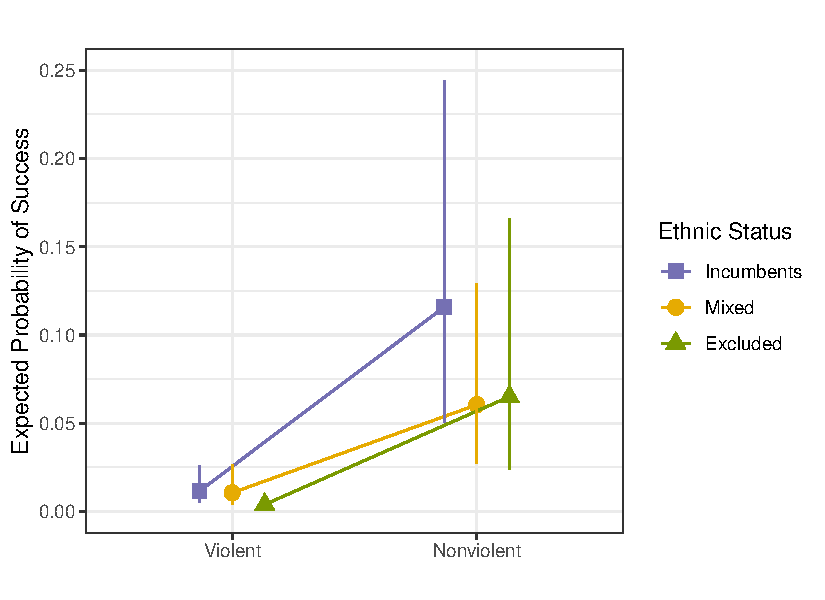
\includegraphics{FinalText_RethinkingEthnicity_files/figure-pdf/Coalition Probability Plot-1.pdf}

}

\caption{Expected probabilities by ethnic power status and tactics
(Model 4).}

\end{figure}%

\subsection{\texorpdfstring{\textbf{A nonviolent advantage at all ethnic
status
levels}}{A nonviolent advantage at all ethnic status levels}}\label{a-nonviolent-advantage-at-all-ethnic-status-levels}

After examining the effect of ethnic power status across tactics, we now
examine the effect of tactics at different ethnic status levels. In both
Models 3 and 4, the use of primarily nonviolent tactics is strongly and
consistently associated with greater likelihood of success. Figure 1
provides a visually compelling illustration of this finding. While the
patterns associated with ethnic power status are statistically
significant, they are substantively overshadowed by the fact that for
all three ethnic status levels, campaigns employing primarily nonviolent
tactics have higher expected likelihoods of success. For example, among
campaigns of only Excluded ethnic groups, Model 4 anticipates a
probability of success of just 0.4\% when primarily violent tactics
used, compared to 6.5\% when primarily nonviolent tactics are used.

To present this another way, Figure 2 shows the pairwise contrasts of
nonviolent as compared to violent tactics, conditional on ethnic power
status. The marginal effects are positive and statistically significant
irrespective of the power status of participating ethnic groups. Across
all power status levels, campaigns that employ primarily nonviolent
tactics are associated with expected success rates between 4 and 10
percentage points higher than those that use violent tactics.

\begin{figure}[H]

{\centering 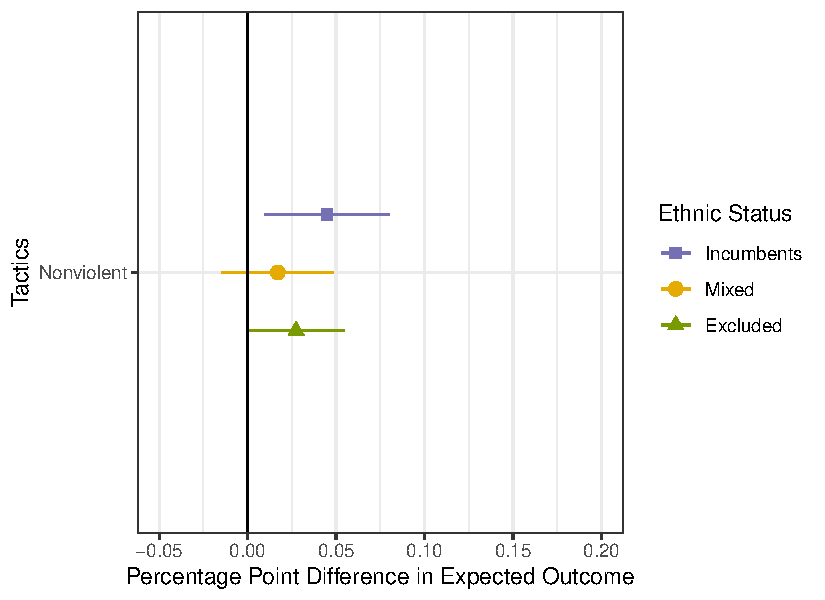
\includegraphics{FinalText_RethinkingEthnicity_files/figure-pdf/Conditional Effects of Nonviolence-1.pdf}

}

\caption{Conditional effects of nonviolent tactics by ethnic power
status (Model 4).}

\end{figure}%

We interpret this as strong support of hypothesis 2, that the use of
primarily nonviolent tactics is associated with higher rates of campaign
success at all ethnic power status levels. Even when facing the greater
obstacles presented by Excluded power status, the use of primarily
nonviolent tactics has historically outperformed the use of violent
tactics in terms of achieving the stated political goals of the
campaign.

Even if nonviolent tactics are associated with higher rates of success
for all ethnic status levels, do they confer a greater advantage for the
privileged than the marginalized? A close look at Figure 1 shows that
the slope of the line for Incumbents appears steeper than that for the
Mixed and Excluded status levels. Indeed, incumbents increase their
likelihood of success by 10 percentage points, from 1\% to 11\% , when
using nonviolent as opposed to violent tactics. Campaigns made up
entirely of excluded groups increase their likelihood of success by only
6 percentage points, from 0.5\% to 6.5\%. But which is actually greater
is a matter of interpretation. The ``smaller'' 6 percentage point jump
for excluded groups actually represents a 13-fold increase in their
likelihood of success. This difference in additive versus multiplicative
interpretations is reflected in our regression models. The interaction
term in Model 4--a logit model based on ``log odds''--is not
statistically significant. By contrast, when we run a linear probability
model as a robustness check in the Appendix (Table 6), it is positive
and significant.

The difference also helps explain one source of variance between our
findings and some from a recent study by Manekin and Mitts (2022).
However, it cannot account for why we find nonviolent tactics to be
positively associated with success among marginalized groups, while they
do not. We conduct further comparisons in the Online Appendix
(pp.~32-34) and conclude that this discrepancy stems primarily from
differences in the underlying data. The updated NAVCO 2.1 dataset
includes additional cases of excluded groups achieving success through
nonviolent tactics that were not included in previous versions.
Additionally, our time-variant approach allows us to more precisely code
cases like the Second Defiance Campaign in South Africa and the East
Timorese independence movement that changed tactics over time. Our data
are able to reflect NAVCO's determinations that these campaigns achieved
success during years in which they used primarily nonviolent tactics.

In the Online Appendix (p.~34), we run models intended to closely
approximate those used by Manekin and Mitts, but using our data. When we
do so, we still find a statistically significant positive effect for
nonviolent tactics when used by minorities. This further increases our
confidence in the empirical support for Hypothesis 2. It is also
consistent with recent findings by Cunningham (2023).

\subsection{\texorpdfstring{\textbf{Diversity helps in nonviolent
campaigns}}{Diversity helps in nonviolent campaigns}}\label{diversity-helps-in-nonviolent-campaigns}

Next. we examine the relationship between diversity and outcomes as
posited in Hypothesis 3. Model 1 shows the expected positive correlation
between the (logged) number of groups participating and the likelihood
of success among nonviolent campaign-years.\footnote{We take the log to
  capture potential diminishing returns to diversity. We expect the
  difference between 1 and 2 groups participating to matter more than
  the difference between 4 and 5.} Interestingly, in Model 2, we see
that no such relationship exists within violent campaign-years. As a
result, Model 4 shows a positive and significant interaction term
between tactics and the (log) number of ethnic groups.

To better illustrate the findings in meaningful terms, Figure 3 presents
the predicted probabilities of campaign success from Model 4, varying
both the number of participating groups and primary tactics. We see that
for nonviolent campaigns, the expected likelihood of success increases
from just 4\% when only 1 group participates, to 8\% when 2 groups are
participating, to 11\% when 5 groups participate. By contrast, the trend
among violent campaigns is nearly flat, with a predicted probability of
success of less than 1\% at all numbers of groups.

\begin{figure}[H]

{\centering 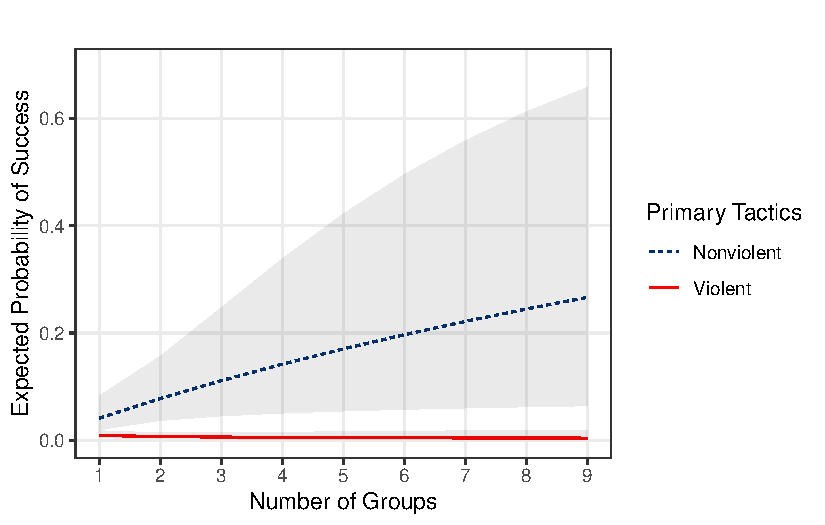
\includegraphics{FinalText_RethinkingEthnicity_files/figure-pdf/Group Probability Plot-1.pdf}

}

\caption{Expected probabilities by number of groups and primary tactics
(Model 4).}

\end{figure}%

\section{Robustness and Sensitivity of the
Findings}\label{robustness-and-sensitivity-of-the-findings}

\subsection{Alternative Measures}\label{alternative-measures}

We further assess the robustness of the findings with additional
measures, models, and analyses. They are presented in full form in an
Online Appendix and discussed briefly here. First, we examine
alternative measures of ethnicity that can be drawn from our dataset. We
use a binary measure of diversity (for any campaign with more than one
ethnic group). We also use a binary measure of ethnic power status,
coding whether or not the ethnic group constituting a plurality of the
participants in a given campaign year is an Incumbent or Excluded group.
This measure more closely approximates measures used in prior studies.
It allows us to assess whether our findings are contingent on our unique
coding of ``Mixed'' status as a distinct category. We use a binary
measure of demographic majority as an alternative measure of group size.
This also reflects a measure similar to one used in previous research
\autocite{Manekin2022}. Finally, we code whether or not a campaign makes
explicit ethnic claims, regardless of its ethnic composition, and assess
this measure as yet another dimension of ethnicity in conflict. While
ethnic claims are highly correlated with the ethnic composition of a
movement, campaign actors may make strategic decisions about whether to
frame their claims in identity-based or more universal framings
\autocite{McLauchlin2017}.

Figure 4 presents a panel of expected probability plots for each of
these alternative measures. They show patterns consistent with our main
findings. In the Online Appendix, we also run models where we exclude
all cases with groups that EPR codes as ``irrelevant.'' Again, the
results are nearly identical. Thus, while a main point of this paper has
been to introduce more complex ways of measuring ethnic dynamics within
conflicts, our findings appear to be robust to alternative measures of
ethnicity, including those used in prior studies.

\begin{figure}[H]

{\centering 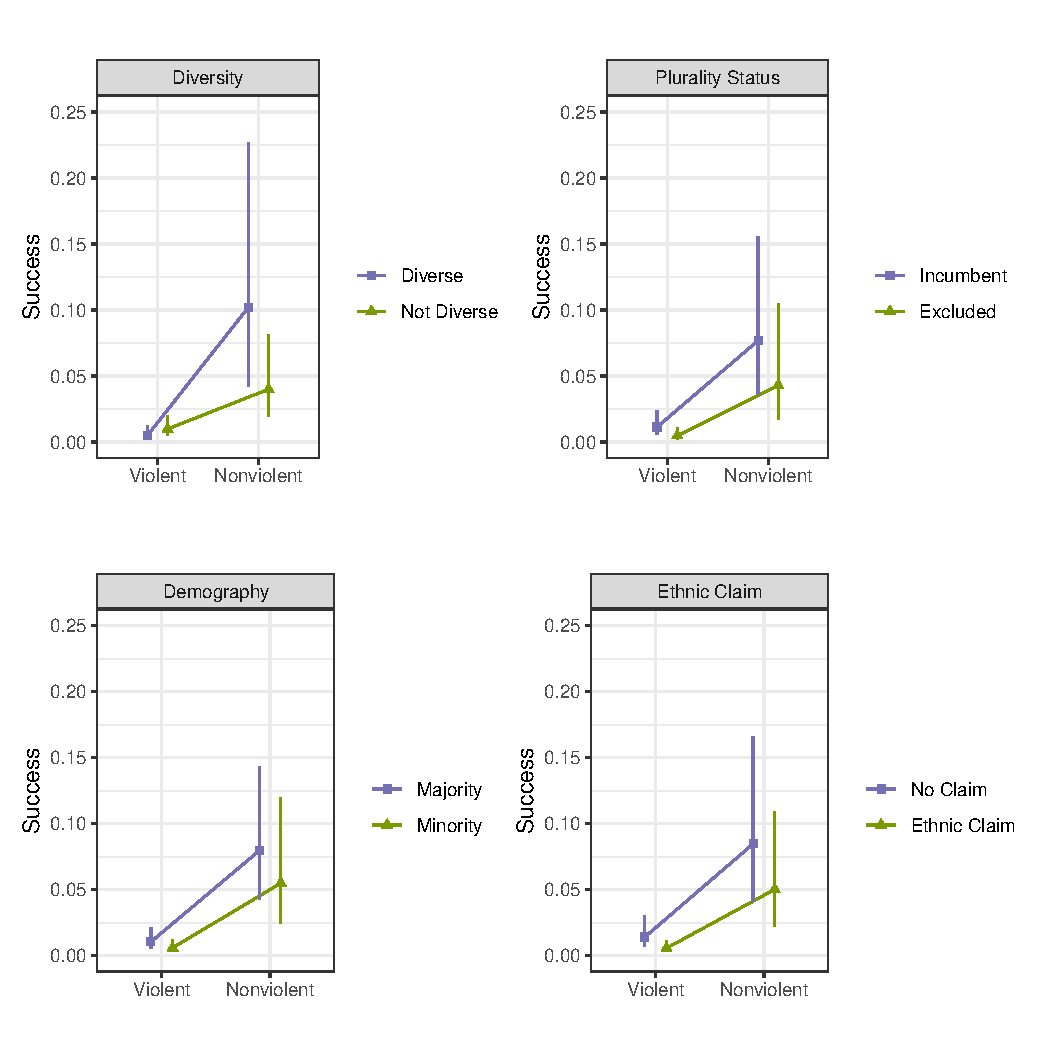
\includegraphics[width=6in,height=6in]{FinalText_RethinkingEthnicity_files/figure-pdf/Alternative Measures Plots, figures-side-1.pdf}

}

\caption{Probability plots using alternative binary measures of ethnic
dimensions.}

\end{figure}%

\subsection{Alternative Modeling
Choices}\label{alternative-modeling-choices}

After exploring different measures of ethnicity, we also test the
robustness of our findings to different model specifications. We run
models on the subset of campaigns seeking regime change to ensure our
findings are not the result of secessionist versus center-seeking goals.
We also run models with additional control variables for simultaneous
campaigns of different tactics, past participation in violent or
nonviolent campaigns, international support, and transnational ethnic
kin. Our results do not change when these variables are included.

Finally, we run year-level, country-level, and two-way fixed effects to
account for potential unobserved confounding variables that could be
correlated with these units. This is a powerful robustness test, as it
effectively controls for a wide array of potential unmeasured
confounding variables associated with country and time, such as colonial
history, past conflict, ethnic demographics, and state capacity. Once
again, the results are nearly identical to those of the main models
presented in Table 4.

\subsection{Selection bias}\label{selection-bias}

The fixed effects models lead us to the next concern, which is the
possibility of endogeneity bias in an observational study. While the
results of the fixed effects models help us rule out omitted variables
that are correlated with time and country, we still worry about the
potential for unmeasured factors that condition movements' prospects for
success and groups' willingness to participate in a resistance campaign
that uses either primarily violent or primarily nonviolent
tactics.\footnote{To even be included in the NAVCO dataset, a campaign
  needs to mobilize at least 1,000 participants, which is itself a
  metric of success. And that threshold might be more or less difficult
  to achieve depending upon tactics used. We consider this as part of
  the types of ``selection effects'' to be examined in this section.}

For the power status measures, members of lower status groups may be
less likely to believe that resistance would be successful and to choose
not to initiate or participate in a resistance campaign. Those that do
anyway could possibly be doing so because they have some other reason to
believe that they are likely to be successful that we are unable to
measure in our models. To put it differently, our set of observed
Excluded cases could be biased in the direction of those that are more
likely to succeed. If this is the case, it would mean that our measured
association between power status and success is an \emph{underestimate}.
In the absence of selection bias, our results would actually be
stronger. We conduct sensitivity analyses for the power status variables
in the appendix as well. It would not take that powerful of an omitted
confounding variable to undo our findings. In fact, the power status
variables already fall just below traditional thresholds of significance
even in our main model for nonviolent campaign-years. But again, we
think that in the absence of selection bias, our findings pertaining to
power status would likely be even stronger.

It is possible that there is both a selection effect for power status as
described above, and that the degree of the selection effect could vary
across violent and nonviolent tactics. If members of Excluded groups
were more likely to be deterred from engaging in nonviolent resistance,
but were nevertheless willing to attempt violent resistance, it would
complicate our ability to interpret the relative association between
tactics and success across ethnic power levels. The low share of
nonviolent campaign-years coded as Excluded as compared to violent
campaign-years is suggestive that this might be the case \autocite[see
also][]{Thurber2018}. Once again, we turn to sensitivity analyses to
assess the vulnerability of our findings to this issue. Because of the
difficulty in interpreting a sensitivity analysis with interaction
terms, we instead run separate models for the set of campaigns falling
into each of the levels of our ethnic status power variable. Most
relevant to our hypotheses, we find that among campaigns made up of only
Excluded groups, unobserved confounding variables would have to explain
more than 11\% of the residual variance in both treatment and outcome to
make the correlation between nonviolent tactics and success no longer
statistically significant. Compared to the strongest confounding
variable included in the model, country population, unmeasured
confounders would have to be more than five times as strong before the
results were no longer statistically significant.

In the case of diversity, we believe the biggest risk may be that when
bystanders see a movement that they perceive as likely to be successful,
they are more likely to participate, thus increasing the number of
different groups participating. To see if this might be the case, we run
models in which we control for campaign size (Online Appendix, p.~22).
When we do so, the relationship between number of groups and success is
no longer significant even within nonviolent campaigns. But the causal
ordering here is not clear. Indeed, part of the logic of our diversity
hypothesis is that greater diversity expands the reach of social
networks available to a campaign making greater mobilization possible.
If so, controlling for campaign size would introduce post-treatment
bias. Further research might wish to more precisely unpack the timing of
campaigns diversity, size, and outcomes.

\section{Expanding Concepts of ``Success'' and
``Nonviolence''}\label{expanding-concepts-of-success-and-nonviolence}

The primary goal of this paper has been to offer a more thorough
analysis of the role of ethnicity in conflict. But the literature on the
outcomes of violent and nonviolent campaigns has frequently been
criticized for oversimplifying both the dichotomy between ``violence''
and ``nonviolence'' as well as between ``success'' and ``failure''
\autocite{Turner2023}. These simplifications may be especially
problematic for the inquiry into the role of ethnicity.

For example, fearing greater repression, minority groups may be more
likely to engage in ``hybrid'' strategies in which protesting masses are
defended by armed flanks, or in which such flanks engage in violent
offensive attacks for greater coercive leverage. The uMkhonto we Sizwe
within the anti-Apartheid movement in South Africa is perhaps the most
prominent example. Meanwhile, even when marginalized groups are not able
to achieve their full goal, obtaining even limited concessions can be
very consequential \autocite{Cunningham2023}. Understanding if and when
groups are able to achieve smaller steps toward progress is an important
outcome that has previously been overlooked.

In this section, we analyze the relationship between ethnicity,
strategy, and campaign outcomes using more precise measures of both
strategy and outcome. First, we use NAVCO 2.1's measure of ``violent
flanks'' to subdivide the category of nonviolent campaigns into
``hybrids'' that included the presence of a flank that used violent
tactics, versus those that maintained more complete nonviolent
discipline. We run an interaction model that parallels that used in our
main analysis (Table 3, Model 4). The results are presented in Figure 5
and in tabular form in the Online Appendix. Figure 5 shows all three
pairwise contrasts within the re-coded 3-level tactics variable for each
level of ethnic status. It shows that the more strictly nonviolent
campaigns and those employing hybrid tactics are largely associated with
similar outcomes: both outperform campaigns that use primarily violent
tactics, though the confidence intervals are now wider as there are
fewer cases within each of the nonviolent factor levels. The results are
largely consistent across ethnic coalition types.

Most noteworthy is the fact that we see no evidence of hybrid tactics
being advantageous to Excluded ethnic groups. Violent flanks are
sometimes argued to be helpful or even necessary for minorities engaging
in nonviolent tactics in order to counter violent regime repression. If
anything, the empirical record appears to show the opposite: our model
estimates lower expected rates of success when Excluded groups
incorporate armed flanks as compared to when they use more strictly
nonviolent tactics, though the difference is not statistically
significant.

\begin{figure}[H]

{\centering 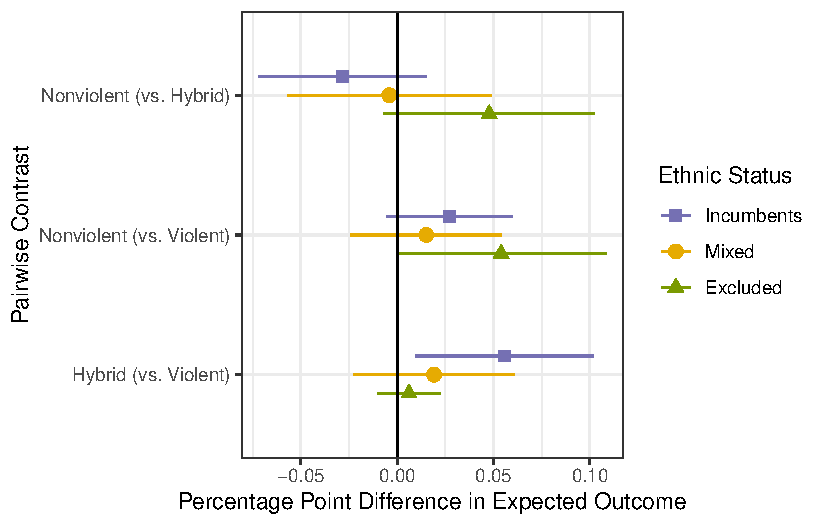
\includegraphics{FinalText_RethinkingEthnicity_files/figure-pdf/flanks contrast plot-1.pdf}

}

\caption{Disaggregating violent flanks.}

\end{figure}%

Next, we use NAVCO 2.1's ``progress'' variable to assess outcomes at
lower thresholds than total victory. We run a series of models on
different outcome thresholds from ``Any progress'' to ``Limited
concessions'' to ``Significant concessions.'' Figure 6 presents the
findings, including our original baseline (Model 3) as a point of
comparison (see also Online Appendix, Table 18). The results show that
as the outcome threshold is lowered, the ethnic attributes of a campaign
make less and less of a difference. In fact, neither of the coalition
variables is significant at any threshold other than the full success
benchmark. While nonviolent strategy is still associated with positive
outcomes at all levels, we see the relationship weaken as the threshold
of success lowers. Challenger coalitions may face longer odds of
achieving total victory, but they are just as likely to achieve more
minor concessions as more privileged groups. Such ``minor'' concessions
could be especially meaningful for members of marginalized and
discriminated groups \autocite{Cunningham2023}.

\begin{figure}[H]

{\centering 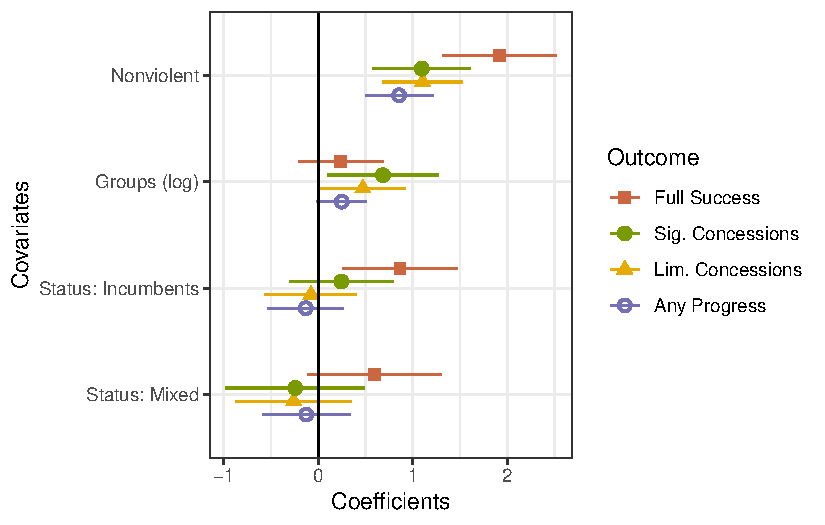
\includegraphics{FinalText_RethinkingEthnicity_files/figure-pdf/Progress-1.pdf}

}

\caption{Lower thresholds of success.}

\end{figure}%

\section{Conclusion}\label{conclusion}

Concerns about the obstacles facing ethnic and racial minorities have
emerged as one of the most important critiques of the supposed
effectiveness of nonviolent tactics. This paper has offered a thorough
reassessment of the observational record on the relationship between
ethnicity, tactics, and outcomes in civil conflicts.

Our results reaffirm the importance of the power status of participating
ethnic groups on campaign outcomes. But they also introduce several
important caveats: power status is associated with outcomes in violent
as well as nonviolent campaigns, and we observe no significant
relationship when examining lower thresholds of success. Most
importantly, we show that even for excluded ethnic groups, nonviolent
tactics are associated with higher rates of success. These findings
should not trivialize the real dangers and challenges facing
marginalized groups engaged in dissent, but they offer an important
rebuttal to an emerging but over-simplified assertion in public
discourse that nonviolent methods ``do not work'' for ethnic minorities.

These results also have important theoretical implications for
understanding the strategic logic of violent and nonviolent conflict. It
upends the presumption made in most prior work that the challenges
facing ethnic minorities are unique to nonviolent action. We think that
those studies accurately identify mechanisms, such as barriers to mass
mobilization and lower likelihood of regime defections, that make
effective resistance more difficult for politically excluded groups. But
armed conflicts may be more reliant on similar mechanisms for success
than we often think. As such, these obstacles to mobilization and
defection yield lower success rates for minority-led armed campaigns. It
might also be the case that commitment problems related to power sharing
among ethnic groups in post-conflict orders make negotiated settlements
more difficult in both violent and nonviolent conflicts.

Our study also calls attention to the varied dimensions of ethnic
identity in conflict and provided new data that make analyses of these
varied dimensions possible. Future research might use this data to
better understand changes in the ethnic composition of campaigns over
time, the relationships among different ethnic groups within a campaign,
demographic attributes of participating ethnic groups, and the ethnic
geography of conflict.

Indeed, we think that the field might benefit from advancing from the
task of measuring the success rates of ethnic minorities in conflict to
understanding the unique strategies that minorities might be able to
employ to make nonviolent tactics more effective for them. For example,
along the lines of a recent study by Manekin, Mitts, and Zeira
\autocite*{Manekin2024}, experimental work might explore how subjects
assess multi-ethnic protest. Or it might seek to manipulate the types of
claims made by protesters in addition to their identities. Case studies
might explore the puzzle of why minority-led movements struggle to
achieve complete success even when they are able to gain significant
concessions from the regime. Are the challenges associated with elite
defection and civil-military relations a greater barrier than obstacles
to early-stage mobilization? Finally, practice-oriented research should
move beyond the general ``playbook'' of civil resistance to identify
strategies that might be particularly effective or necessary for
campaigns by marginalized ethnic groups.

\section{Acknowledgements}\label{acknowledgements}

The authors would like to thank Chris Butler, Cassy Dorff, Jonathan
Pinckney, and participants in presentations at the Korbel Research
Seminar at Denver University, the Four Corners Conflict Network, and the
2023 International Studies Association Annual Meeting for helpful
feedback. We would also like to thank JPR editors and three anonymous
reviewers for construtive suggestions that improved this manuscript.

\section{Funding information}\label{funding-information}

Presentation of an earlier version of this manuscript at the 2023 ISA
Annual Meeting in Montreal, Canada was supported, in part, by a grant
from the Institute for Human Studies at George Mason University
(No.~IHS016972).

\section{Data Availability Statement}\label{data-availability-statement}

The dataset, codebook, and scripts for the empirical analysis in this
article, along with the Online Appendix, are available at
https://www.prio.org/jpr/datasets/\ldots{} as well as at
www.chesthurber.com. All analyses were conducted using R.


\printbibliography[title=References]



\end{document}
